\graphicspath{{Chapter2/Figs/}}

\section{Multi-Omics Factor Analysis: a framework for unsupervised integration of multi-omics data sets}
% In the first section of this chapter, we will describe XXX

The work described in this chapter results from a collaboration with the Multi-omics and statistical computing group lead by Wolfgang Huber at the EMBL (Heidelberg, Germany). It has been peer-reviewed and published in Argelaguet \& Velten et al \cite{Argelaguet2018}.\\

The method was conceived by Florian Buettner, Oliver Stegle and me. I performed most of the mathematical derivations and implementation, but with significant contributions from Damien Arnol and Britta Velten. The single-cell application was led by me whereas the CLL data application was led by Britta Velten, but with joint contributions in either cases. Florian Buettner, Wolfgang Huber and Oliver Stegle supervised the project.\\
The article was jointly written by Britta Velten, Florian Buettner, Wolfgang Huber, Oliver Stegle and me.


\subsection{Model description}
MOFA is a multi-view generalisation of traditional Factor Analysis to $M$ input matrices (or views) $\bfY^m \in \R^{N \times D_m}$ based on the framework of Group Factor Analysis (discussed in Section X).\\
The input data consists on $M$ views with non-overlapping features that often represent different assays. However, there is flexibility in the definition of views and they can be tailored to address different hypothesis.\\
%For example, if one has DNA methylation data, one could define as a single view the matrix with all genome-wide measurements, but one could also split this matrix into different views, either by chromosome or by genomic context (i.e. promoters, enhancers, etc.).\\
Formally, the input data is factorised as:
\begin{equation}
	\mathbf{Y}^m = \mathbf{Z}\mathbf{W}^{mT} + \bepsilon^m
\end{equation}
where $\bfZ \in \R^{N \times K}$ is a matrix that contains the factor values and $\bfW^m \in \R^{D_m \times K}$ are $M$ matrices that contain the loadings that relate the high-dimensional space to the low-dimensional latent representation. Finally, $\bepsilon^m \in \R^{D_m}$ captures the residuals, or the noise, which is assumed to be normally distributed and heteroskedastic:
\begin{equation}
	p(\epsilon^m_d) = \Ndist{\epsilon^m_d}{0,1/\tau_d^m}
\end{equation}
Non-gaussian noise models can also be defined and is discussed in Section XX. Unless otherwise stated, we will always assume Gaussian noise.\\
Altogether, this results in the following likelihood:
\begin{equation}
	p(\bfY|\bfW,\bfZ,\bTau) = \prod_{m=1}^{M} \prod_{d=1}^{D_m} \prod_{n=1}^{N} \Ndist{y_{nd}^m}{\bfz_{n}^T\bfw_{d}^{m},1/\tau_d^m}
	% p(y_{nd}^m) = \Ndist{y_{nd}^m}{\bfz_{n,:}\bfw_{d,:}^{mT},1/\tau_d^m},
\end{equation}

\subsubsection{Interpretation of the factors}
Each factor ordinates cells along a one-dimensional axis centered at zero. Samples with different signs indicate opposite phenotypes, with higher absolute value indicating a stronger effect. For example, if the $k$-th factor captures the variability associated with cell cycle, we could expect cells in the Mitosis state to be at one end of the factor (irrespective of the sign, only the relative positioning being of importance). In contrast, cells in G1 phase are expected to be at the other end of the factor. Cells with intermediate phenotype, or with no clear phenotype (i.e. no cell cycle genes profiled), are expected to be located around zero, as specified by the prior distribution.

\subsubsection{Interpretation of the loadings}
The loadings provide a score for each gene on each factor, and are interpreted in a similar way as the factors. Genes with no association with the factor are expected to have values close to zero, as specified by the prior. In contrast, genes with strong association with the factor are expected to have large absolute values. The sign of the loading indicates the direction of the effect: a positive loading indicates that the feature is more active in the cells with positive factor values, and viceversa. \\
Following the cell cycle example from above, we expect genes that are upregulated in the M phase to have large positive loadings, whereas genes that are downregulated in the M phase (or, equivalently, upregulated in the G1 phase) are expected to have large negative loadings.\\

% The following figure shows a real-case example of a Factor capturing the cell cycle effect, with the corresponding loadings:

% \begin{figure}[H]
% 	\begin{center}
% 		\includegraphics[width=1.0\textwidth]{figures/cell_cycle}
% 		\caption{Example of a factor (Factor 2) that captures the cell cycle phenotype. Left shows a scatterplot of Factor 1 and Factor 2, where each dot is a single cell. The cells are colored by the infered lineage and they are shaped by the infered cell cycle phase. Right shows the RNA expression loadings for Factor 5. Each dot represents a gene.  }
% 		\label{fig:cell_cycle}
% 	\end{center}
% \end{figure}


\subsubsection{Interpretation of the noise}
The use of a probabilistic framework allows the model to explicitly disentangle the signal (i.e. the explained variance) from the noise (i.e. unexplained variance). Large values of $\tau_d^m$ indicate high certainity on the observations for the feature $d$ in view $m$, as predicted by the latent variables. In contrast, small values of $\tau_d^m$ are indicative of low predictive power by the latent variables.

\subsubsection{Missing values}
The probabilistic formalism naturally accounts for incomplete data matrices, as missing observations do not intervene in the likelihood.\\
In practice, we implement this using memory-efficient binary masks $\mathcal{O}^m \in \mathbb{R}^{N\times D_m}$ for each view $m$, such that $\mathcal{O}_{n,d} = 1$ when feature $d$ is observed for sample $n$, 0 otherwise. 

\subsubsection{Prior distributions for the factors and the loadings}
The key determinant of the model is the regularization used on the prior distributions of the factors and the weights.\\
For the factors, we follow common practice \cite{XX} and define an isotropic Gaussian prior:
\begin{equation}
	p(z_{nk}) = \Ndist{z_{nk}}{0,1}
\end{equation}
For the weights we encode two levels of sparsity, a (1) view- and factor-wise sparsity and (2) an individual feature-wise sparsity. The aim of the factor- and view-wise sparsity is to disentangle the activity of factors to the different views, such that the weight vector $\bfw_{:,k}^m$ is shrunk to zero if the factor $k$ does not explain any variation in view $m$. \\
In addition, we place a second layer of sparsity which encourages inactive weights on each individual feature. Mathematically, we express this as a combination of an Automatic Relevance Determination (ARD) prior \cite{Mackay1996} for the view- and factor-wise sparsity and a spike-and-slab prior \cite{Mitchell1988} for the feature-wise sparsity:
% \begin{equation*}
% 	p(w_{dk}^{m}) = (1-\theta_{k}^{m}) \mathds{1}_0(w_{dk}^{m}) + \theta_{k}^{m} \Ndist{w_{dk}^{m}}{0, 1 / \alpha_{k}^{m}}
% \end{equation*}
However, this formulation of the spike-and-slab prior contains a Dirac delta function, which makes the inference procedure troublesome. To solve this we introduce a re-parametrization of the weights $w$ as a product of a Gaussian random variable $\hat{w}$ and a Bernoulli random variable $s$, \cite{Titsias2011} resulting in the following prior:
% \begin{equation}
% 	p(\hat{w}_{dk}^m,s_{dk}^m) &= \Ndist{\hat{w}_{dk}^m}{0, 1/\alpha_k^m}  \text{Ber}(s_{dk}^m \,|\,\theta_k^m)
% \end{equation}
In this formulation $\alpha_k^m$ controls the activity of factor $k$ in view $m$ and $\theta_k^m$ controls the corresponding fraction of active loadings (i.e. the sparsity levels).\\

Finally, we define conjugate priors for $\theta$ and $\alpha$:
\begin{align}
	p(\theta_k^m) &= \Bdist{\theta_k^m}{a_0^\theta,b_0^\theta}\\
	p(\alpha_k^m) &= \Gdist{\alpha_k^m}{a_0^\alpha, b_0^\alpha},
\end{align}
with hyper-parameters $a_0^\theta,b_0^\theta =1$ and $a_0^\alpha, b_0^\alpha=1e^{-3}$ to get uninformative priors.\\
Posterior values of $\theta_k^m$ close to $0$ implies that most of the weights of factor $k$ in view $m$ are shrinked to $0$ (sparse factor). In contrast, a value of $\theta_k^m$ close to $1$ implies that most of the weights are non-zero (non-sparse factor). A small value of $\alpha_k^m$ implies that factor $k$ is active in view $m$. In contrast, a large value of $\alpha_k^m$ implies that factor $k$ is inactive in view $m$.\\

All together, the joint probability density function of the model is given by
\begin{align}
	\begin{split}
	p(\bfY,\hat{\bfW},\bfS,\bfZ,\btheta, \balpha, \btau)  = &\prod_{m=1}^{M} \prod_{n=1}^{N} \prod_{d=1}^{D_m} \Ndist{y_{nd}^m}{\sum_{k=1}^{K} s_{dk}^m \hat{w}_{dk}^m z_{nk},1/\tau_d} \\
	& \prod_{m=1}^{M}\prod_{d=1}^{D_m} \prod_{k=1}^{K} \Ndist{\hat{w}_{dk}^m}{0,1/\alpha_k^m} \text{Ber}(s_{d,k}^m|\theta_k^m) \\
	& \prod_{n=1}^{N} \prod_{k=1}^{K} \Ndist{z_{nk}}{0,1} \\
	& \prod_{m=1}^{M} \prod_{k=1}^{K} \Bdist{\theta_k^m}{a_0^\theta,b_0^\theta}\\
	& \prod_{m=1}^{M} \prod_{k=1}^{K} \Gdist{\alpha_k^m}{a_0^\alpha, b_0^\alpha}\\
	& \prod_{m=1}^{M} \prod_{d=1}^{D_m} \Gdist{\tau_d^m}{a_0^\tau,b_0^\tau}.
	\label{likelihood}
	\end{split}
\end{align}
and the corresponding graphical model is shown in \Cref{fig:MOFA_graphical_model}. This completes the definition of the MOFA model.

\subsection{Downstream analysis}

Once trained, the MOFA model can be queried for a set of downstream analysis:
\begin{itemize}
	\item \textbf{Variance decomposition}: calculate the variance explained ($R^2$) by each factor in each view. 
	\item \textbf{Ordination of the samples in the latent space}: scatterplots or beeswarm plots of factors, colored or shaped by sample covariates can reveal the main drivers of sample heterogeneity.
	\item \textbf{Inspection of loadings}: the weights (or loadings) can be interpreted as an activity score for each gene on each factor. Hence, inspecting the top loadings reveals the genes (or other genomic features) that underlie each factor.
	\item \textbf{Imputation}: MOFA generates a condensed and denoised low-dimensional representation of the data without missing values. As discussed in Section X, the data can be reconstructed from the latent space by a simple matrix multiplication: $\hat{\bfY} = \bfZ \bfW^T$. 
	\item \textbf{Feature set enrichment analysis}: when a factor is difficult to characterise based only on the inspection of the top loadings, one can compute a statistical test for enrichment of biological pathways using predefined gene-set annotations. The statistical tests that we implemented are outlined in Section X.
\end{itemize}

The downstream functionalities implemented in MOFA are highlighted in \Cref{fig:MOFA}.

\begin{figure}[H]
	\begin{center}
		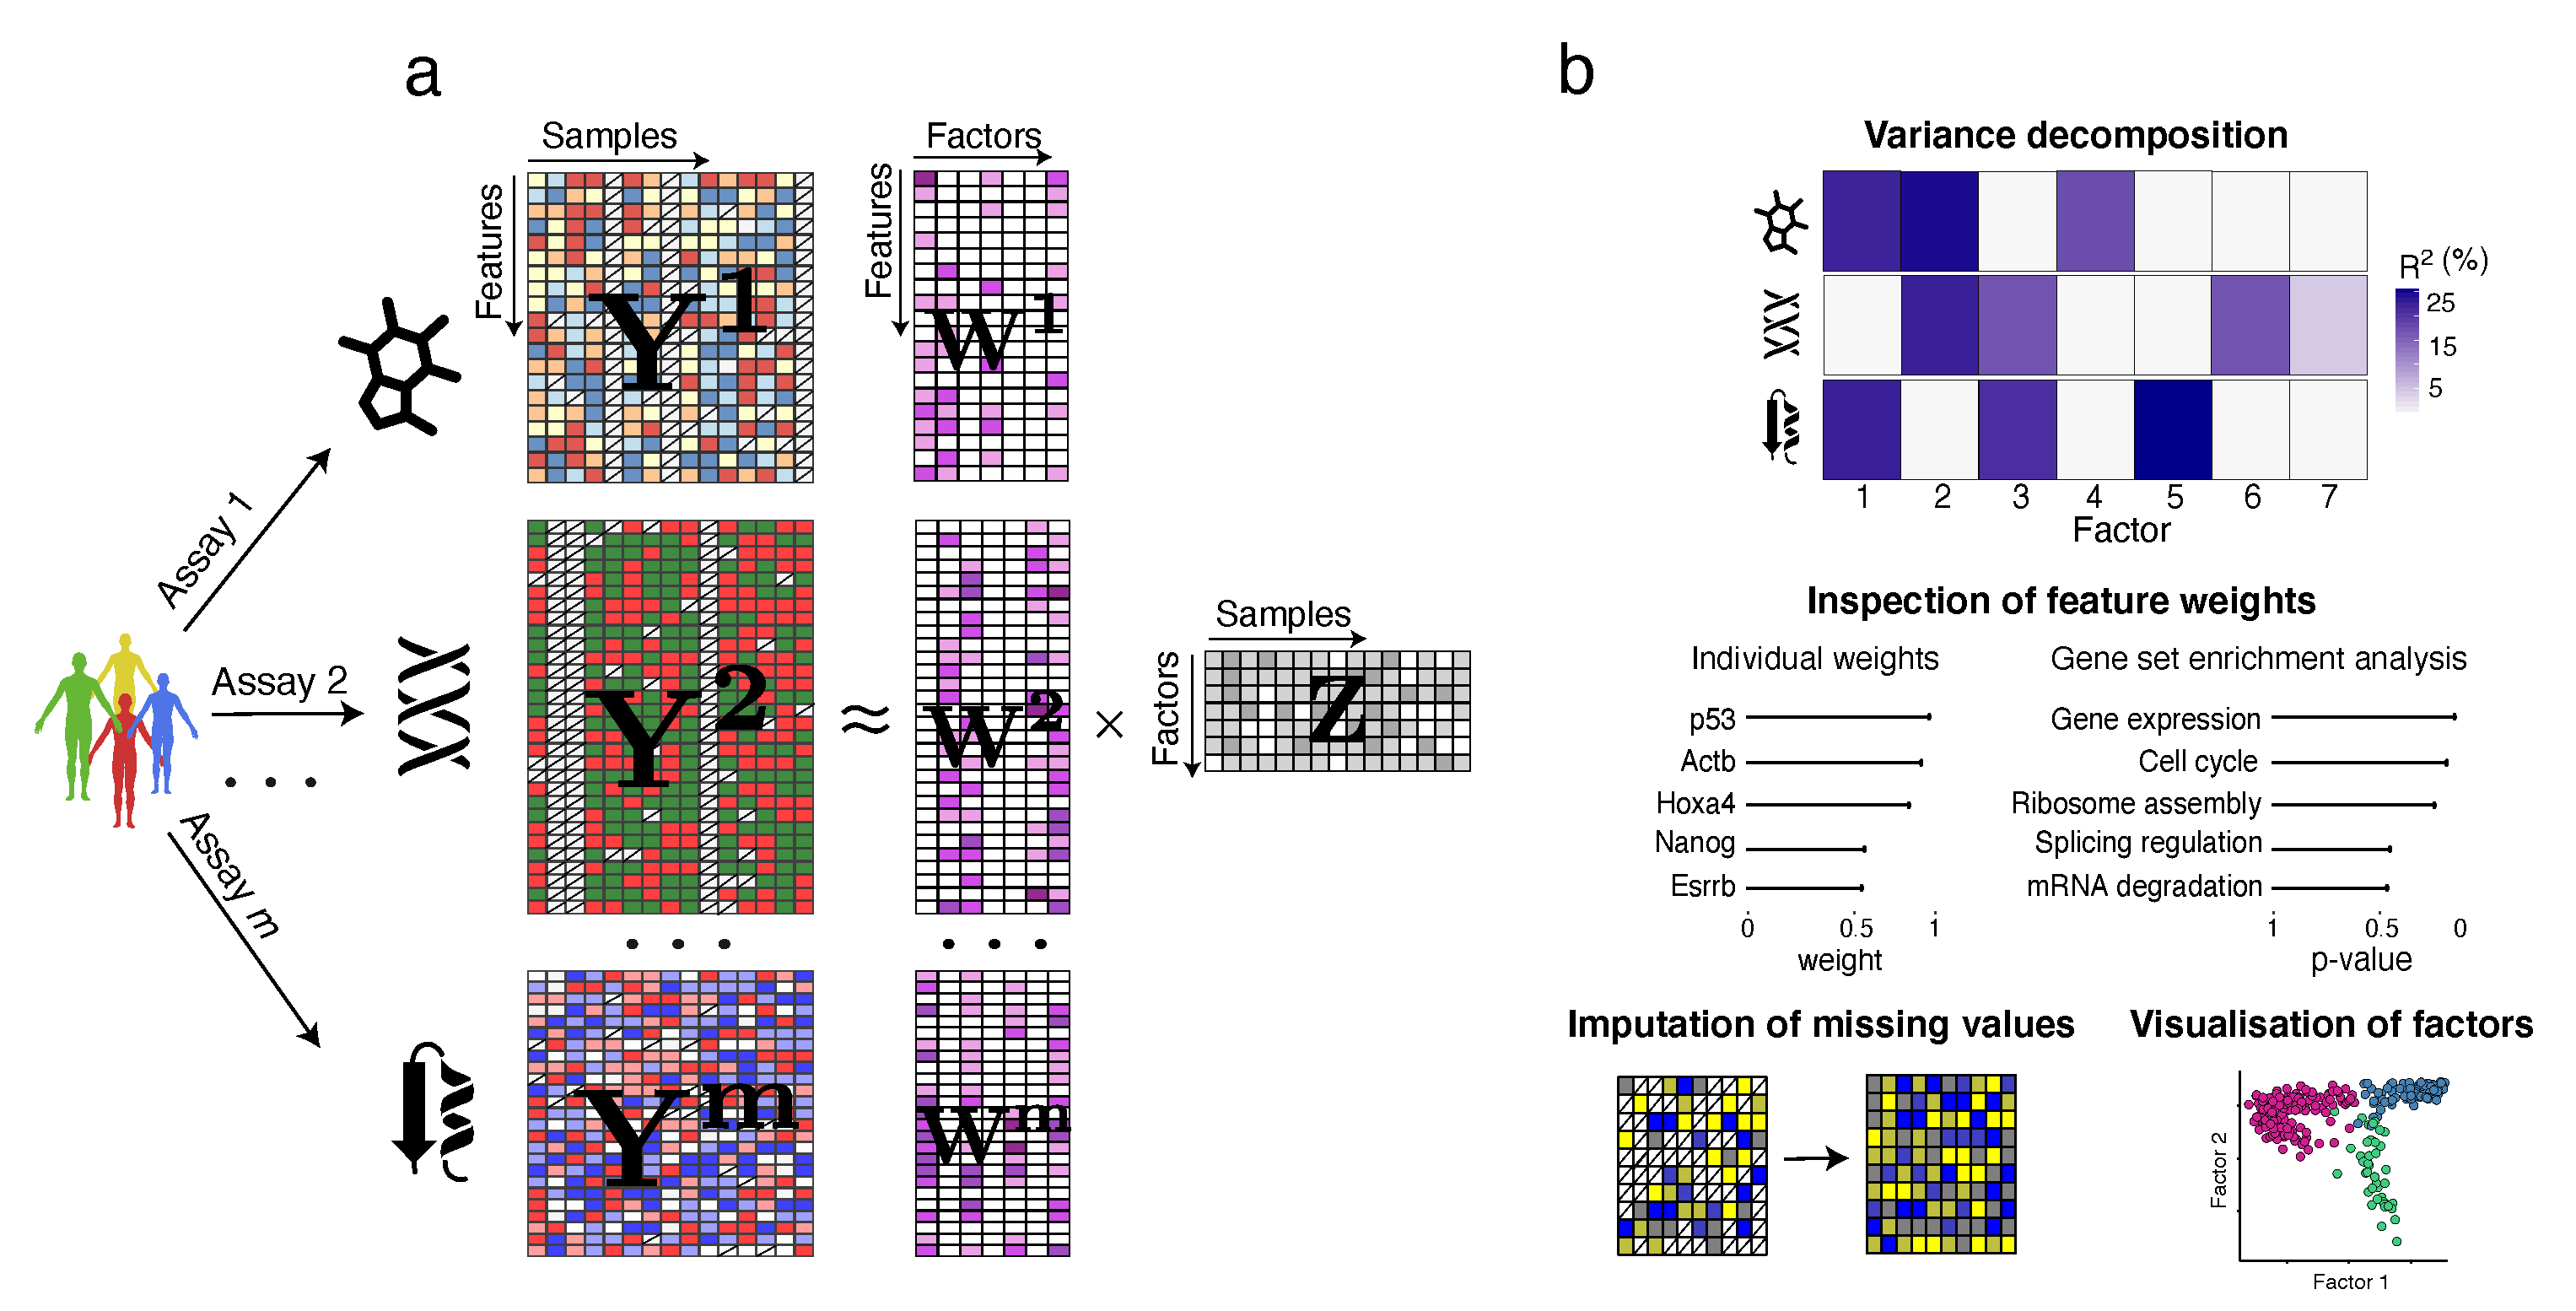
\includegraphics[width=1.0\textwidth]{MOFA}
		\caption{MOFA overview. The model takes $M$ data matrices as input ($\bfY^1, \cdots, \bfY^M$), one or more from each data modality, with co-occurrent samples but features that are not necessarily related and can differ in numbers. MOFA decomposes these matrices into a matrix of factors ($\bfZ$) and $M$ weight matrices, one for each data modality ($\bfW^1, \cdots, \bfW^M$). White cells in the weight matrices correspond to zeros, i.e. inactive features, whereas the cross symbol in the data matrices denotes missing values. The fitted MOFA model can be queried for different downstream analyses, including a variance decomposition to assess the proportion of variance explained by each factor in each data modality.}
		\label{fig:MOFA}
	\end{center}
\end{figure}

\begin{figure}[H]
	\centering
	% \definecolor{colD}{rgb}{0.2, 0.2, 0.6}
\definecolor{colM}{rgb}{0.0, 0.5, 0.0}
\definecolor{colN}{rgb}{0.5, 0.0, 0.13}
\definecolor{colG}{rgb}{1.0, 0.65, 0.0}
\newcommand\op{0.25}
\colorlet{shadecolor}{black!25}

\newcommand\op{0.25}

\begin{tikzpicture}
  % Define nodes:
  % matrix factorisation level
  \node[obs]   (Y) {$y_{n,d}^m$};
  \node[latent, above=of Y, xshift=-1.5cm] (Z) {$z_{n,k}$};
  \node[latent, above=of Y, xshift=1.5cm] (W) {$w_{k,d}^m$};
  \node[latent, xshift=1.5cm] (Tau) {$\tau_{d}^m$};

  % \node[opacity=\op,latent, xshift=-1.5cm] (Tau2) {$\tau_{n}$};

  % parents of Z
  \node[opacity=\op, det, above=of Z] (crossZ) {$\times$};
  \node[opacity=\op, latent, above=of crossZ] (Zhat) {$\hat{z}_{n,k}^{\ }$};
  \node[opacity=\op, latent, above=of Zhat] (SigmaZ) {$\alpha_k$};
  \node[opacity=\op, latent, above=of crossZ, xshift=-1.5cm] (SZ) {$s_{n,k}$};
  \node[opacity=\op, latent, above=of SZ] (ThetaZ) {$\theta_{k}$};

  % parents of W
  \node[det, above=of W] (crossW) {$\times$};
  \node[latent, above=of crossW] (What) {$\hat{w}_{k,d}^m$};
  \node[latent, above=of What] (SigmaW) {$\alpha_k^m$};
  \node[latent, above=of crossW, xshift=1.5cm] (SW) {$s_{k,d}^m$};
  \node[latent, above=of SW] (ThetaW) {$\theta_{k}^m$};

  % Connect the nodes
  \edge {Z,W, Tau} {Y}; %
  \edge[opacity=\op] {ThetaZ} {SZ};
  \edge[opacity=\op] {SigmaZ} {Zhat};
  \edge {ThetaW} {SW};
  \edge {SigmaW} {What};
  % \edge[opacity=\op] {Tau2} {Y}

  \factoredge[opacity=\op] {SZ, Zhat} {crossZ} {Z};
  \factoredge {SW, What} {crossW} {W};

  % cluster plate
  % \node[latent, above=of What, xshift=-1.3cm, opacity=0.15] (muW) {$\mu^m_{k, c}$};
  % \node[latent, above=of Zhat, xshift=1.3cm, opacity=0.15] (muZ) {$\mu_{k, c}$};
  % \edge[opacity=\op] {muZ} {Zhat};
  % \edge[opacity=\op] {muW} {What};
  % \plate[] {plateC} {(muZ)(muW)} {$C$};

  % Plates
  % \plate[] {plateK} {(Z)(W)(SZ)(Zhat)(SW)(What)(ThetaZ)(ThetaW)} {$K$};
  % \plate[color=colN, fill=colN, fill opacity=0.1] {plateN} {(Y)(Z)(crossZ)(Zhat)(SZ)(plateK.south west)} {\color{colN} $N$};
  % \plate[color=colD ,fill=colD, fill opacity=0.1] {plateD} {(Y)(W)(Tau)(crossW)(What)(SW)(plateK.south east) (plateN.south east)} {\color{colD}$D_m$};
  % \plate[color=colM,fill=colM, fill opacity=0.1] {plateM} {(plateD)(ThetaW)(plateK.north east)} {\color{colM}$M$};
  \plate[] {plateK} {(Z)(W)(SZ)(Zhat)(SW)(What)(ThetaZ)(ThetaW)} {$K$};
  \plate[] {plateN} {(Y)(Z)(crossZ)(Zhat)(SZ)(plateK.south west)} {$N$};
  \plate[] {plateD} {(Y)(W)(Tau)(crossW)(What)(SW)(plateK.south east) (plateN.south east)} {$D_m$};
  \plate[] {plateM} {(plateD)(ThetaW)(plateK.north east)} {$M$};

\end{tikzpicture}

	\caption{Graphical model for MOFA. The white circles represent hidden variables that are infered by the model, whereasa the grey circles represent the observed variables. There are a total of four plates, each one representing a dimension of the model: $M$ for the number of views, $N$ for the number of samples, $K$ for the number of factors and $D_m$ for the number of features in view $m$}
	\label{fig:MOFA_graphical_model}
\end{figure}

\subsubsection{Inference}
To make the model scalable to large data sets we adopt a Variational inference framework with a structured mean field approximation. 
A detailed overview is given in section XX, and details on the variational updates for the MOFA model are given in Appendix XX.\\
To enable efficient inference for non-Gaussian likelihoods we employ local bounds \cite{XX}. This is described in detail in Section X

\subsection{Monitoring convergence}
An attractive property of Variational inference is that the objective function, the Evidence Lower Bound (ELBO), is required to monotonically increase at every iteration. This provides a simple way of monitoring convergence \Cref{fig:elbo_convergence}. This is indeed one of the reasons why we selected this inference framework over Expectation Propagation or sampling-based approaches.

 \begin{figure}[H]
	\centering 	
	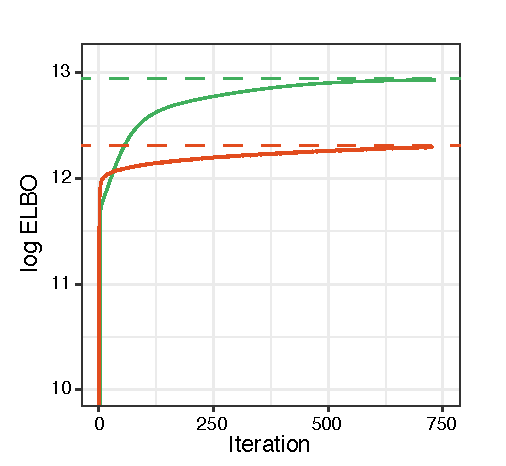
\includegraphics[width=0.5\textwidth]{elbo_convergence}
	\caption{XX}
	\label{fig:elbo_convergence}
\end{figure}

\subsection{Model selection and consistency across random initilizations} \label{section:robustness}
The optimisation problem in MOFA is not convex and the algorithm is not guaranteed to find the optimal solution \cite{XX}. Therefore, posterior distributions will vary depending on the initialisation and it becomes mandatory to perform model selection and assess the consistency of the factors across different trials.\\

The strategy we follow here is to train several MOFA models (e.g. 10 trials) under different parameter initialisations, and subsequently select the model with the highest ELBO for downstream analysis. In addition, we evaluate the robustness of the factors by plotting the Pearson correlations between factors across all trials. \Cref{fig:MOFA_robustness}. 

A similar strategy has also been proposed in \cite{Hore2016}.


\begin{figure}[H]
	\centering 	
	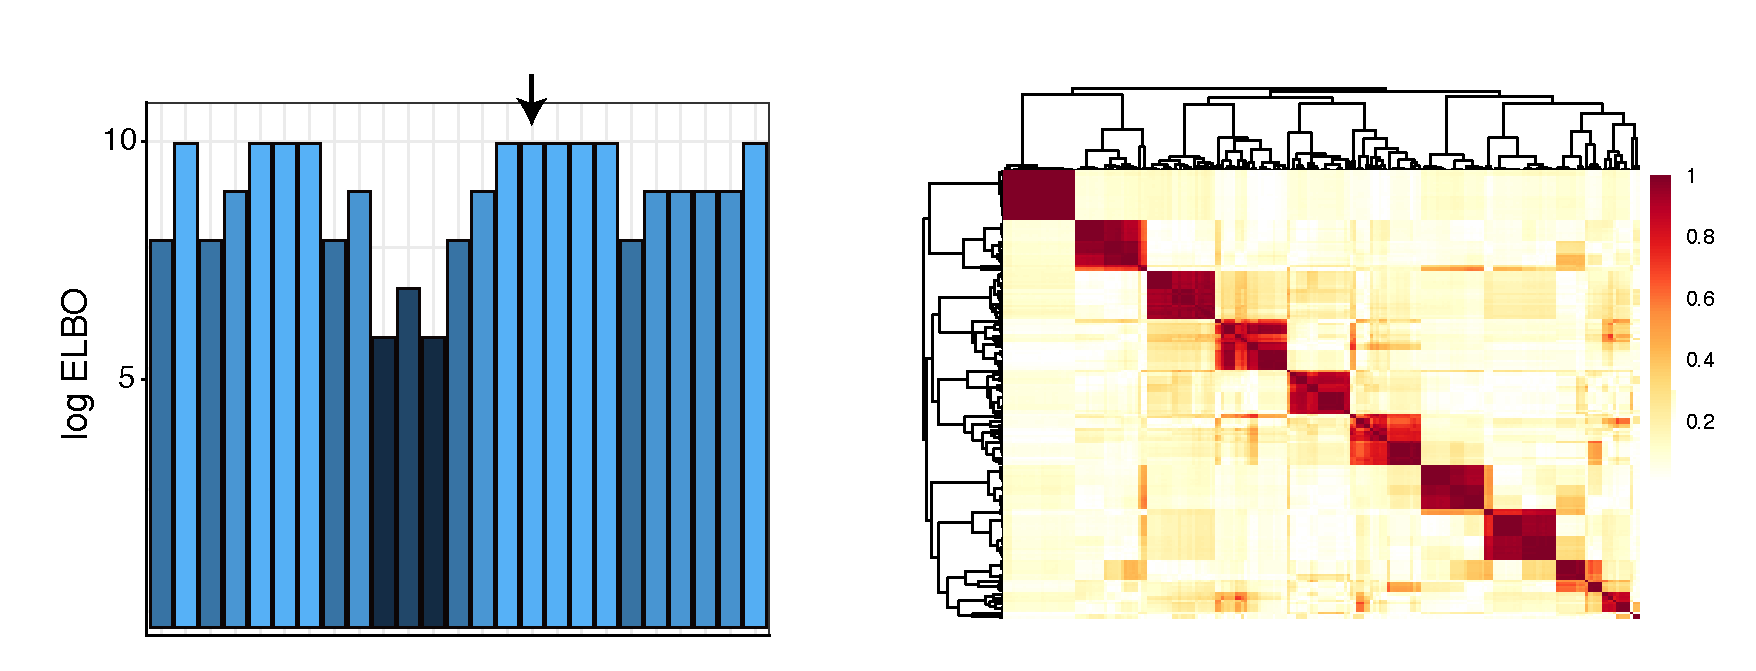
\includegraphics[width=1.0\textwidth]{MOFA_robustness}
	\caption{XX... A block-diagonal matrix ensures good consistency across random initialisations}
	\label{fig:MOFA_robustness}
\end{figure}


% \subsection{Feature Set Enrichment Analysis}

% \subsection{Comparison with previous methods}

%The key difference with the sparse Bayesian factor analysis model in Section XX is that we learn a separate $\alpha_k^m$ and $\theta_k^m$ per factor and view, instead of per factor. This allows the model to take into account that the data is structured into different views.\\



\subsection{Learning the number of factors} \label{section:number_factors}
As described in section X, the use of an ARD prior allows factors to be actively prunned by the model if they explain negligible variation. In the implementation this is controlled by a hyperparameter that defines a threshold on the minimum fraction of variance explained by a factor (across all views).\\
Additionally, because of the non-convexity of the variational inference algorithm, different model instances can potentially yield solutions with different number of active factors (\Cref{fig:mofa_nfactors}). The optimal number of factors need to be selected by the model selection strategy outlined in \Cref{section:robustness}.

\begin{figure}[H]
	\centering 	
	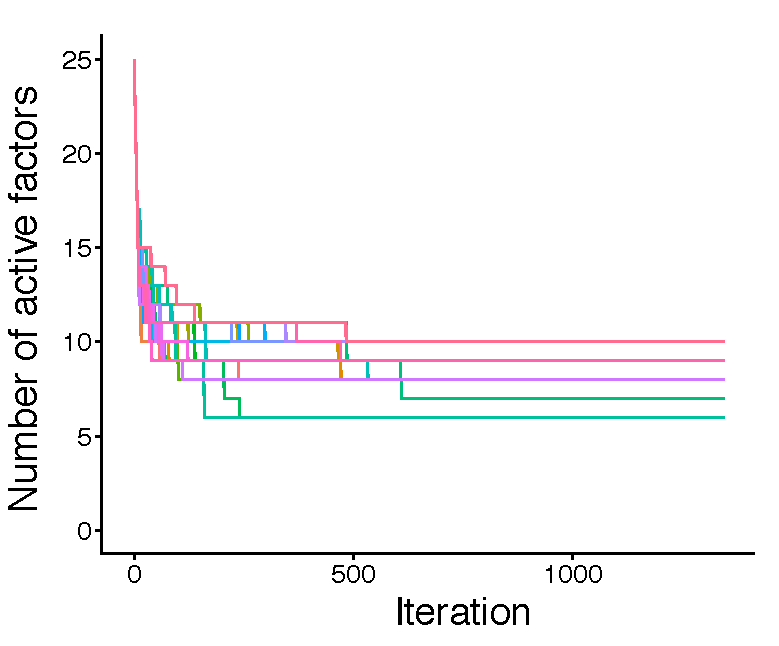
\includegraphics[width=0.5\textwidth]{MOFA_nfactors}
	\caption{XX}
	\label{fig:MOFA_nfactors}
\end{figure}



\subsection{Application to single-cell multi-omics} \label{section:mofa_scmt}

The emergence of single-cell multi-modal techniques has created open opportunities the development of novel computational techniques that integrate data sets across multiple modalities \cite{XX}. Here, we investigated the potential of MOFA to unravel the heterogeneity in one of the earliest single-cell multi-omics data sets \cite{Angermuelller2016}.\\
The data set consists on 87 embryonic stem cells (ESCs) where RNA expression and DNA methylation were simultaneously profiled using single-cell Methylation and Transcriptome sequencing (scM\&T-seq).
Two populations of ESCs were profiled: the first one contains 16 cells grown in 2i media, which induces a native pluripotency state with genome-wide DNA hypomethylation \cite{XX}. the second population contains 71 cells grown in serum media, which triggers a primed pluripotency state poised for differentiation \cite{XX}.\\

The RNA expression data was processed using standard pipelines \cite{Lun2016} to obtain log normalised counts, followed by a selection of the top 5,000 most overdispersed genes \cite{XX}.\\
The DNA methylation data was processed as described in section XXX. Briefly, for each CpG site, we calculated a binary methylation rate from the ratio of methylated read counts to total read counts. Next, CpG sites were classified by overlapping with genomic contexts, namely promoters, CpG islands and enhancers (defined by the presence of distal H3K27ac marks). Finally, for each annotation we selected the top 5,000 most variable CpG sites with a minimum coverage of 10\% across cells.\\
Each of the resulting matrices was input as a separate view to MOFA.\\

In this data set, MOFA learnt 3 factors (minimum explained variance of 2\%). Factor 1 captured the transition from naive to primed pluripotent states, which MOFA links to widespread coordinated changes between DNA methylation and RNA expression. Inspection of the gene loadings for Factor 1 pinpoints important pluripotency markers including  Rex1/Zpf42 or Essrb \cite{XX}. As previously described both in vitro (Angermueller et al, 2016) and in vivo (Auclair et al, 2014), the dynamics of DNA methylation are driven by a genome-wide increase in DNA methylation levels \cite{XX}

Factor 2 captured a second axis of differentiation from a primed pluripotency state to a differentiated state (Figure 6b,c).
e to a differentiated state with highest RNA loadings for known differentiation markers such as keratins and annexins

% Interestingly, the combination of Factors 1 and 2 captured the entire differentiation trajectory from naive pluripotent cells via primed pluripotent cells to differentiated cells, (Figure 6b), illustrating the importance of learning continuous latent factors rather than discrete sample assignments as done by popular methods such as SNF [47] or iCluster [31,

 %Finally, Factor 3 captured the cellular detection rate, a known tech- nical covariate associated with cell quality and mRNA content (Finak et al, 2015; Appendix Fig S22).

%Jointly, Factors 1 and 2 captured the entire differentiation trajec- tory from naive pluripotent cells via primed pluripotent cells to dif- ferentiated cells (Fig 5E), illustrating the importance of learning continuous latent factors rather than discrete sample assignments. Multi-omics clustering algorithms such as SNF (Wang et al, 2014) or iCluster (Shen et al, 2009; Mo et al, 2013) were only capable of distinguishing cellular subpopulations, but not of recovering contin- uous processes such as cell differentiation (Appendix Fig S23).

\begin{figure}[H]
	\centering 	
	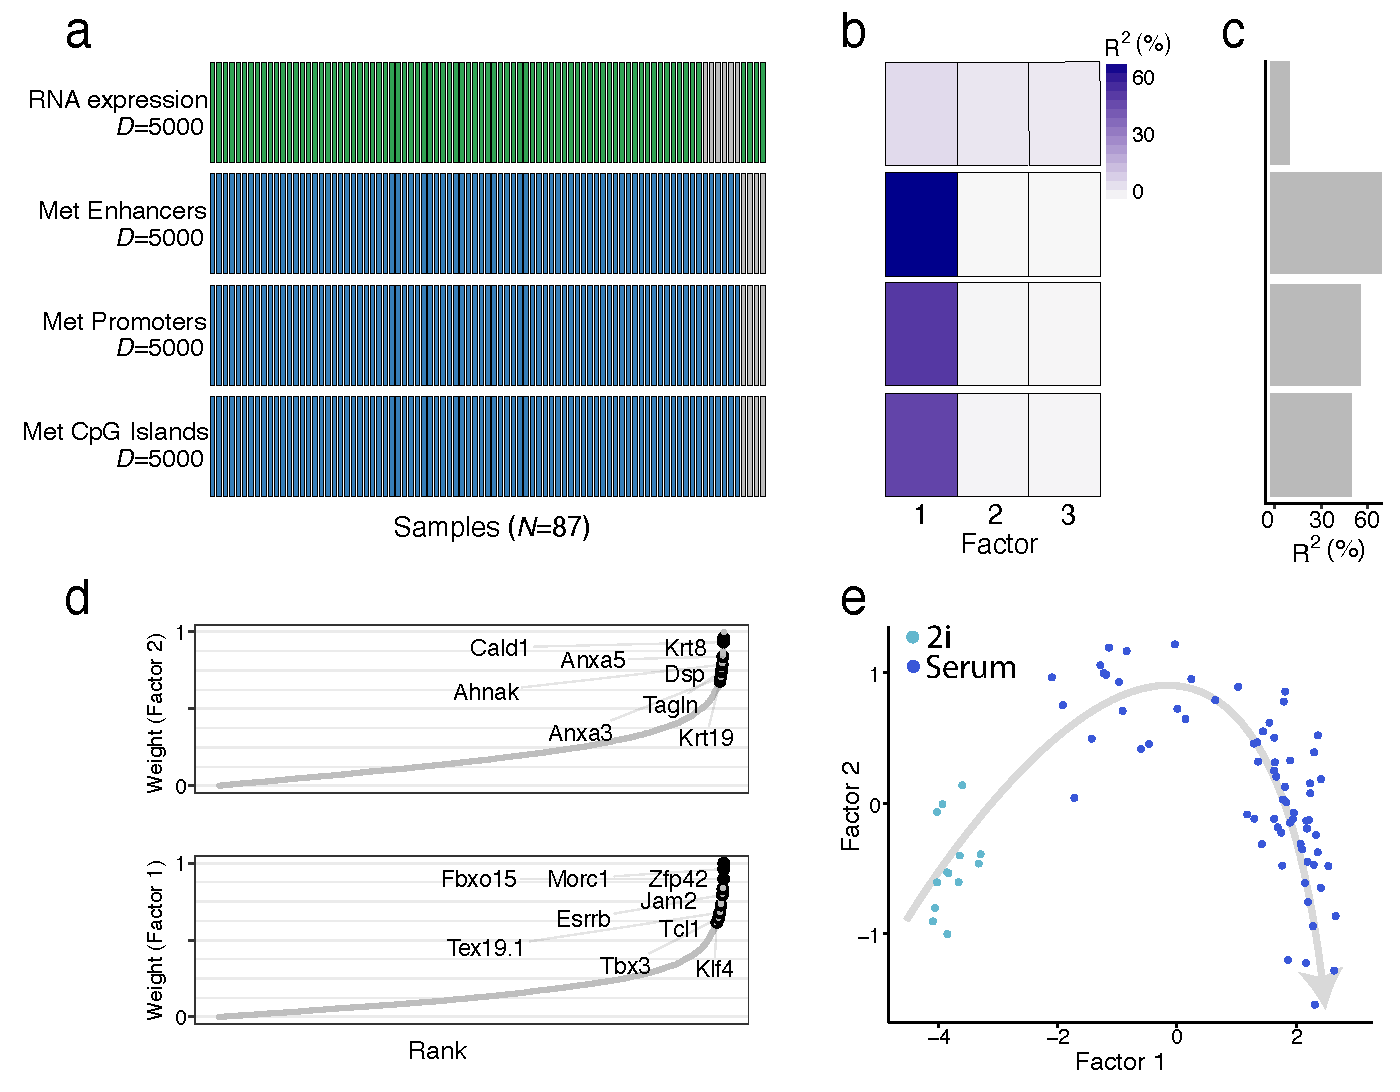
\includegraphics[width=1.0\textwidth]{MOFA_scMT}
	\caption{XX}
	\label{fig:MOFA_scMT}
\end{figure}

% Conclusion: MOFA reveals coordinated changes between the transcriptome and the epigenome along a differentiation trajectory

\subsection{Open perspectives}
% We developed Multi-Omics Factor Analysis (MOFA), an unsupervised method for decomposing the sources of heterogeneity in multi-omics data sets. We illustrated its potential using two data sets with high- dimensional and incomplete multi-omics profiles.
% Although we have addressed important challenges for multi-omics applications, MOFA is not free of limitations. The model is linear, which means that it can miss strongly non-linear relationships between features within and across views. Non-linear extensions of MOFA may address this, although as with any models in high-dimensional spaces, there will be trade-offs between model complexity, computational efficiency and interpretability [14]. Also, a related area of work is to incorporate prior information on the relationships between individual features [6]. Finally, while here we use approximate Bayesian inference and focus attention on the resulting point estimates of inferred factors, future extensions could attempt a more comprehensive Bayesian treatment that propagates evidence strength and estimation uncertainties for diagnostics and downstream analyses [46].

% Although we have addressed important challenges for multi- omics applications, MOFA is not free of limitations. The model is linear, which means that it can miss strongly non-linear relation- ships between features within and across assays (Buettner & Theis, 2012). Non-linear extensions of MOFA may address this, although, as with any models in high-dimensional spaces, there will be trade- offs between model complexity, computational efficiency and inter- pretability (preprint: Damianou et al, 2016). A related area of work is to incorporate prior information on the relationships between individual features. For example, future extensions could make use of pathway databases within each omic type (Buettner et al, 2017) or priors that reflect relationships given by the “dogma of molecular biology”. In addition, new likelihoods and noise models could expand the value of MOFA in data sets with specific statistical prop- erties that hamper the application of traditional statistical methods, including zero-inflated data (i.e. scRNA-Seq; Pierson & Yau, 2015) or binomial distributed data (i.e. splicing events; Huang & Sangui- netti, 2017). Finally, while here we focus our attention on the point estimates of inferred factors, future extensions could attempt a more comprehensive Bayesian treatment that propagates evidence strength and estimation uncertainties to diagnostics and down- stream analyses.